

\subsubsection{Specific Temperature Change Method}
Introduced by Radel, Wilson et. al., the Specific Temperature Change method uses 
a linear approximation to arrive at the thermal loading density limit.  
When the thermal time constant of the rock is much shorter than the waste form 
decay package, the change in package wall temperature can be described by 

\begin{align}
\Delta T_1 &= q(t_0)\rho_{limit}C'
\intertext{where}
\Delta T_1 &= T_{lim} - T_{amb} \nonumber\\
T_{lim} &= \mbox{ Temperature limit }[^{\circ}C]\nonumber\\
T_{amb} &= \mbox{ Ambient rock temperature }[^{\circ}C]\nonumber\\
q(t_0) &= \mbox{ Heat at the inital time} \nonumber \\
\rho_{limit} &= \frac{C_1}{Q_1}\nonumber\\
C' &= \mbox{ Thermal constant }[-]\nonumber\\
\Delta T &= T_{lim}-T_{amb}[^{\circ}C]\nonumber\\
\end{align}

\begin{figure}[htp!]
\begin{center}
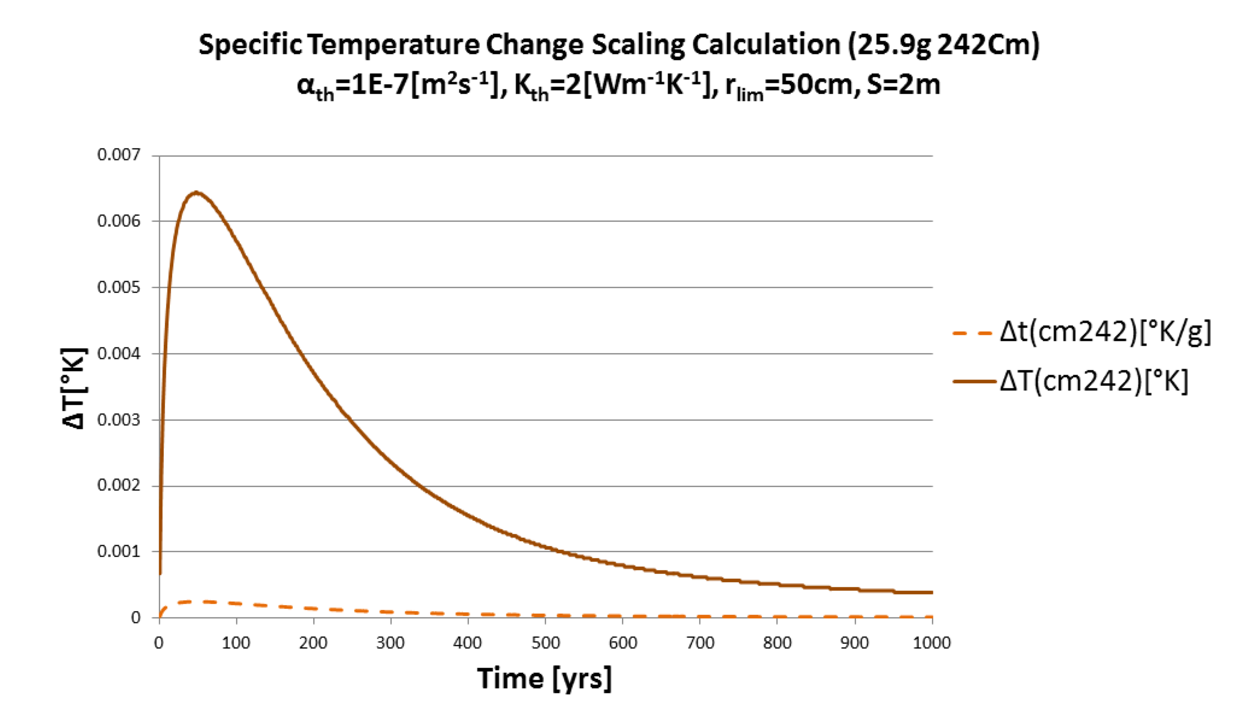
\includegraphics[width=\columnwidth]{images/CmScaling.eps}
\end{center}
\caption{As a demonstration of the calculation procedure, the temperature change 
  curve for one intial gram of $^{242}Cm$ and is scaled to represent $25.9g$, 
  approximately the $^{242}Cm$ inventory per MTHM in 51GWd burnum UOX PWR fuel. }
\label{fig:CmScaling}
\end{figure}

Figure \ref{fig:CmScaling} demonstrates the scaling of an STC curve to represent 
the heat from $25.9g$ of initial $^{242}Cm$. For an arbitrary waste stream 
composition, scaled curves calculated in this manner can be superimposed for 
each heat generating isotope to arrive at an approximate total temperature 
change at the calculation radius. This is demonstrated in figure 
\ref{fig:fakeArbitraryWF}.

\begin{figure}[htp!]
\begin{center}
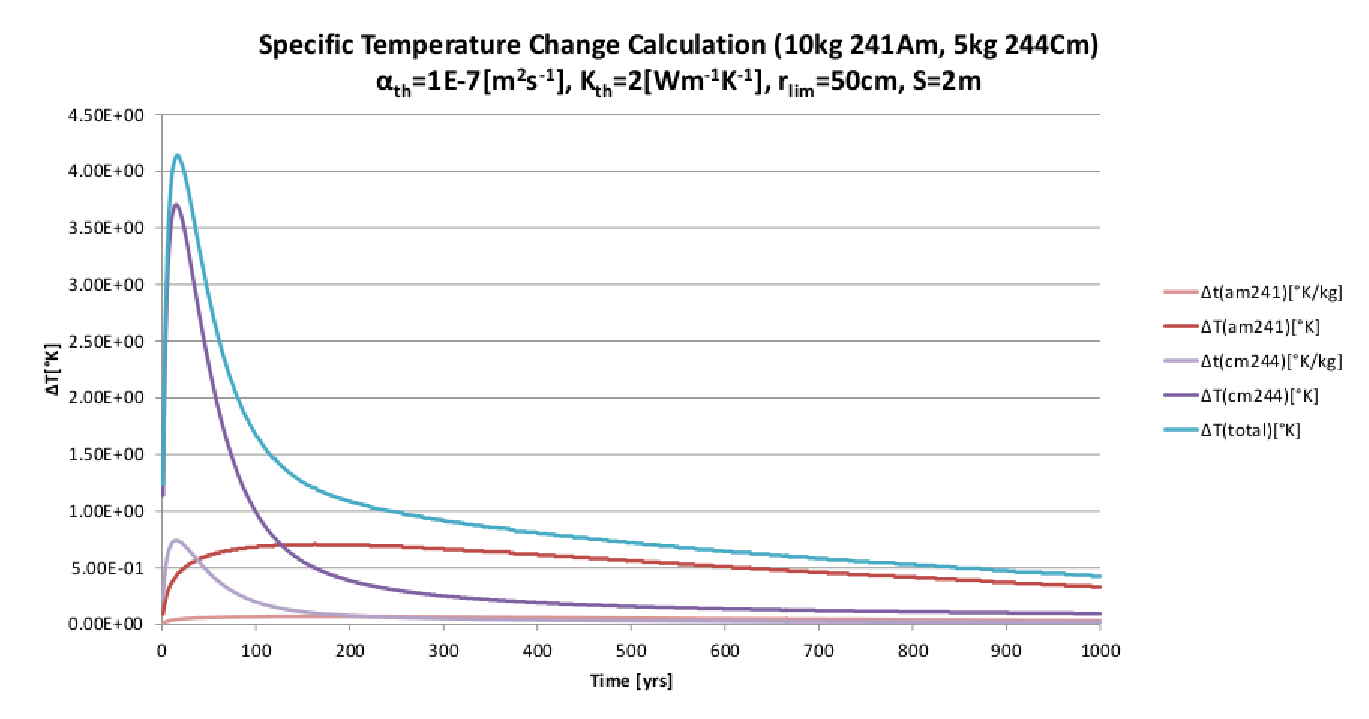
\includegraphics[width=\columnwidth]{images/fakeArbitraryWF.eps}
\end{center}
\caption{As a demonstration of the calculation procedure, scaled temperature change 
  curves for two isotopes are superimposed to achieve a total temperature 
change.}
\label{fig:fakeArbitraryWF}
\end{figure}

To support this calculation in Cyder, a reference data set of temperature change 
curves, $\Delta t_i$, were calculated for high heat contributing isotopes. These 
curves were calclated as a function of specified repository spacing, $S$, heat 
limit radius, $r_{lim}$, and thermal paramters $\alpha_{th}$ and $K_{th}$. The 
total temperature change is the sum of the mass scaled curves,

\begin{align}
\Delta T &\sim \sum_{i\in H} m_i \Delta t_i(r,S,K_{th},\alpha_{th})
\intertext{where}
\Delta T &= \mbox{ total temperature change in waste }[^{\circ}K]\nonumber\\
H &= \mbox{ set of high heat isotopes }[-]\nonumber\\
m_i &= \mbox{ mass of isotope i  } [g]\nonumber\\
\Delta t_i(r,S,K_{th},\alpha_{th}) &= \mbox{ temperature change due to 1 g of i }[^{\circ}K]\nonumber
\label{superposition}
\end{align}
\begin{table}[ht!]
\centering
\footnotesize{
\begin{tabular}{|l|l|l|r|}
\multicolumn{4}{c}{\textbf{Thermal Cases}}\\
\hline
\textbf{Parameter} & \textbf{Symbol} & \textbf{Units} & \textbf{Value Range} \\
\hline
Diffusivity & $\alpha_{th}$ & $[m^2\cdot s^{-1}]$ & $1.0\times10^{-7}-3.0\times10^{-6}$\\
\hline
Conductivity & $K_{th}$     & $[W\cdot m^{-1} \cdot K^{-1}]$ & $0.1 - 4.5$ \\
\hline
Spacing & $S$ & $[m]$ & 2, 5, 10, 15, 20, 25, 50 \\
\hline
Radius & $r_{lim}$ & $[m]$ & 0.1, 0.25, 0.5, 1, 2, 5 \\
\hline
Isotope & $i$ & $[-]$ & $^{241,243}Am,$  \\
        & & & $^{242,243,244,245,246}Cm,$  \\
        & & & $^{238,240,241,242}Pu$  \\
        & & & $^{134,135,137}Cs$  \\
        & & & $^{90}Sr$  \\
\hline
\end{tabular}
\caption{A thermal reference dataset of \gls{STC} values as a function of each of these parameters was generated by repeated parameterized runs of the LLNL 
MathCAD model\cite{greenberg_application_2012, greenberg_investigations_2012}.}
\label{tab:thermal_cases}
}
\end{table}



Repeated runs of a detailed analytic model over the range of values in Table 
\ref{tab:thermal_cases} have given a dataset that 
facilitates estimation of thermal loading capacity for a range of thermal 
diffusitivities, conductivities, and repository layouts. Simple linear 
interpolation across the discrete parameter space provides a simple thermal 
reference dataset for use in Cyder.
